\documentclass{article} 
\usepackage{todonotes}
\usepackage{graphicx}
\usepackage[font=small,labelfont=bf]{caption}
\usepackage[bottom=1.3in]{geometry}
\graphicspath{ {images/} }


\title{URL-Shortener}
\author{Francesco Balzano}


\begin{document}
  \pagenumbering{gobble}
  \maketitle
  \newpage
  \tableofcontents
  \newpage
  \pagenumbering{arabic}
  
\section{Overview}  
URL shortening is the translation of a long Uniform Resource Locator (URL) into an abbreviated alternative that redirects to the longer URL.  A shortened URL may be desired for messaging technologies that limit the number of characters in a message, for reducing the amount of typing required if the reader is copying a URL from a print source, for making it easier for a person to remember, or for the intention of a permalink.\\  
The aim of this project is to provide the implementation of a distributed url-shortener service.


\section{Design choices}
There are three fundamental metrics in the assessment of a distributed system: Consistency, Availability and Partition Tolerance. It is well known from the CAP theorem that it is impossibile to achieve all of them at the same time in a distributed system. \\ 
In this project, I have chosen to focus on availability and partition tolerance, at the expense of consistency. In particular, the consistency model is not a strong one.
In the following subsections, I list and explain the design choices that I made.


\subsection{API}
The url-shortener project is a service that provides the following APIs:

\paragraph{get}
Given the shorten url returns the original url, if present. \\
\texttt{get(shortUrl) -$>$ longUrl}

\paragraph{put}
Generates and returns the shortened url associated with the provided url. \\
\texttt{put(longUrl) -$>$  shortUrl}

\paragraph{remove}
Removes the couple \texttt{<shortened url, original url>}.\\
\texttt{remove(shortUrl) -$>$  longUrl}


\subsection{Passive Replication}
Clients can communicate with every node. If the contacted node is the primary for that request, it will execute the request and directly return the result to the client; otherwise it will forward the request to the primary, which will execute it and send back the response to the sending node, which in turn will hand it back to the client. \\

I have chosen the Passive Replication strategy because I think it should keep lower the number of version conflicts.

\subsection{Data Partitioning}
The partitioning strategy to map objects into nodes is a dynamic one: namely, it is employed Consistent Hashing with virtual nodes. The use of virtual nodes has potentially two advantages: in case of heterogeneous machines we can assign more virtual nodes to the most powerful machines, so that it will be more likely that these machines will handle a bigger number of items. The other advantage concerns homogeneous machines (\texttt{i.e.} machines with similar computational power, bandwidth, storage...). In this case the use of virtual nodes results in a more fair distribution of items among nodes with higher probability. \\ In case of node leave, due for instance to node crash or network partition, the keys asssigned to this node are automatically assigned to another, working node. Since we have replication of data and we use the gossip protocol to detect dead nodes, we are capable to face the leave of one or more nodes without compromising the functioning of the whole system. In other words, availability and partition tolerance are guaranteed.

\subsection{Data Replication}
We want to achieve availability, so an asynchronous replication strategy is adopted. Namely, the primary node immediately answers to the client after an operation is performed. Messages to the backup nodes are sent periodically, and not after every update of the primary's data. This strategy reduces the latency of the communication client-primary, again at the expense of consistency. \\
Each primary node is associated 1 backup node, which is the next node clockwise in the ring. Every time a primary wishes to update its replica, it sends all the content of its database to this node. 

\subsection{Primary Failure}
The use of Consistent Hashing and the the specific data replication strategy adopted (backup is the next node clockwise in the ring) allows to have a vry easy failover procedure: if node \textit{i} is down, the space of keys that belonged to node \textit{i} will be automatically mapped to node \textit{(i+1) mod n}. Since node \textit{(i+1) mod n} is the backup of node \textit{i} it will have a copy of the keys of node \textit{i} (although possibly not updated), so the correct behaviour will be maintained also in case of failure of the primary without needing an explicit failover procedure. For further details about the failover procedure please refer to the  \textit{Implementation} section.    


\subsection{Consistency Model}
This project adopts an eventual consistency model. \todo{In realtà tutte le richieste arrivano a un leader}It is possible to get different results if running the same query at the same time on the leader and on a follower. This may happen if the follower has an outdated version of the leader's data. Anyway this is only a temporary state: if we stop writing to the database for a while, the followers will eventually become consistent with the leader. I decided to accept this weak consistency model in order to have better availability and partition tolerance. 

\subsection{Conflicts Resolution}
Each node is assigned a vector clock that allows it to order events, that is to track causal dependencies between events. When a message is sent from a node to another, it carries both the object (the target of the communication) and the sender's vector clock. If the recipient node already has that object with the associated vector clock in its database, two situations may arise:
\begin{itemize}
\item  If one vector clock is smaller than the other, keep the greatest (i.e. latest) version of the object;
\item  \todo{Non ti puoi affidare al client per risolvere inconsistenze, va fatto server-side}If that is not the case, the two vector clocks are concurrent, and if the two objects are assigned different values then we have a conflict.
\end{itemize}



\section{Implementation}  
There are clients, that invoke the service, and nodes, that comprise the cluster and actually implements the service. Clients and nodes stay in two different modules: the formers in the client module, the latters in the core module. Indeed they are logically different things, and so they should be able to evolve independently from each other. 

\subsection{Architecture} 

The client can make a request to any node in the cluster. The nodes process the request and handle back the result to the client. \todo{Molto specifico, inseriscilo negli use cases?} In particular, only the primary node for a given request actually processes it. If a node receives a request for which it is not the primary, it discovers who is the primary and forwards the request to such node. The primary node processes the request and then handles back the result to the previous node, who in turn returns the response to the client. \\
Each node has to do three main jobs, so I created a node as a container of three services: 
\begin{itemize}
\item \textit{client communication service}: each node must be able to communicate with the client, to accept requests from it and return responses;
\item \textit{node communication service}: each node must be able to communicate with the other nodes. Indeed, it could have to forward the client request to the primary node, or to send the content of its own database to the backup node, or even only to check that the other nodes of the cluster are alive;
\item \textit{storage service}: each node must have a database, to store and retrieve urls on client's behalf. Actually, it has two databases: its own database, used to handle requests, and the backup database, used to replicate the data of another node. The reason for the use of two distinct databases is explained in \textit{``The core module''} paragraph. 
\end{itemize}
Figure \ref{fig:architecture} shows the architecture of the service. The communication between client and nodes exploits TCP, both because I assume an unreliable communication channel between them and because of \textit{interactive} sessions. Indeed the possibility of starting an interactive service session between the client and a node amortizes TCP overhead, since the same amount of overhead will be payed (to open and close the connection) no matter how many times the service is invoked by the client. Instead, communication among nodes in the cluster uses UDP for the opposite reasons. First, I assume a much more reliable network inside the cluster (with respect to Internet, for instance). Second, usually single messages are sent from a node to another, and so establishing a TCP connection to send only one message would be too costly.

\begin{figure}[h]
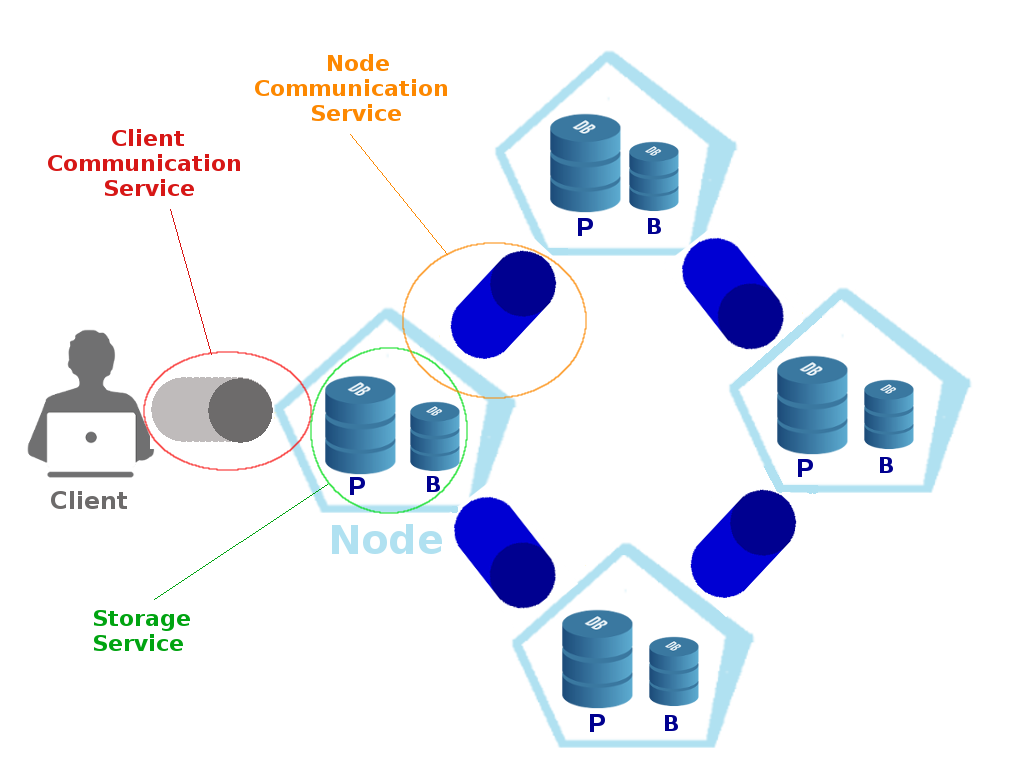
\includegraphics[scale=0.41]{architecture}
\caption{General architecture. There is a client and a cluster, which is made of more nodes. Each node is made of a node communication service, a client communication service and a storage service. The letter ``P'' under the database stays for ``primary'' , the letter ``B'' for ``backup''.}
\label{fig:architecture}
\end{figure}

\subsection{The project classes} 
The structure of the project is the following. The node is the building block of the cluster and, as we already said, it is made of three main \textit{services}. Each of these services provides a high level view of the functionalities it has to implement. For the actual implementation these services rely on proper \textit{managers}, which have the responsability to setup things and handle lower level details. Figure \ref{fig:class_diag} shows a simplified UML class diagram, in which the relationships among classes are highlighted (but not the methods). In particular, this diagram only shows the classes of the \textit{core} module, because it is this module that implements the logic of the service. Instead the \textit{client} module only parses the user's request and sends it to proper classes of the core module to be processed. \\




\subsubsection{The core module} 
The core module contains all the classes that implement the logic of the project. The Node class is the main class and the building block of the cluster. This module contains classes and methods to receive and process client requests, find the primary node for any request, handle the partition and replication of data, cope with node failure and resolve conflicts. Classes inside this module are organized into the following packages: \textit{communication, message, storage} and \textit{utils}. Some classes belong to the \textit{core} package but not to any of the mentioned subpackages. I start describing these classes, and then I pass to the classes in the subpackages. \\
\begin{itemize}
\item \textit{NodeRunner} It is the class that actually runs the url-shortener service. Indeed it setups the cluster by setting the configurations specified in the configuration file. The \textit{main} method of the core package is in this class.
\item \textit{CoreCommandLineManager} Parses the command-line input and provides methods to deal with the options that can be specified from command-line.
\item \textit{Node} It is the building block of the whole cluster. A cluster is a collection of interacting nodes. In turn, each node is made of three services: a \textit{ClientCommunicationService} to handle the communication with the client, a \textit{NodeCommunicationService} to handle the communication with other nodes and a \textit{StorageService} to deal with database operations internal to each node. 
\item \textit{Service} A simple \textit{Interface} for the various services, that only states that each service must provide a \textit{start()} and a \textit{shutdown()} method.
\end{itemize}

\paragraph{Communication} The Communication package gathers classes that are involved in the communication either with clients or with other nodes. For this reason, the classes inside this package are organized in two further subpackages \textit{client} and \textit{node}. 
\subparagraph{Client} 
\begin{itemize}
\item \textit{ClientCommunicationService} One of the three fundamental services a node is made of. It starts and shuts down a ClientCommunicationManager.
\item \textit{ClientCommunicationManager} It listens on a TCP ServerSocket to accept client requests. As soon as a request is received, a ClientCommunicationThread is created and run to handle it. Then, the ClientCommunicationManager continues to listen on the socket for further requests. It also provides a method to process the client request, by delegating the processing to the NodeCommunicationManager.
\item \textit{ClientCommunicationThread} It communicates with the client by using the socket received from ClientCommunicationManager. In particular, it receives the client message, asks the ClientCommunicationManager to process it and finally returns the result to the client.
\end{itemize}
\begin{figure}[h]
\centering
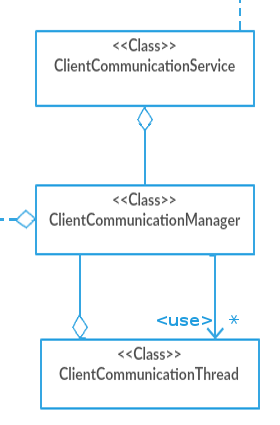
\includegraphics[scale=0.35]{classes_client_subpackage}
\caption{Part of the UML class diagram, showing up relationships among classes in the core.communication.client subpackage}
\label{fig:class_diag_core.communication.client	}
\end{figure}

\subparagraph{Node} 
\begin{itemize}
\item \textit{NodeCommunicationService} One of the three fundamental services a node is made of. It starts and shuts down a NodeCommunicationManager.
\item \textit{NodeCommunicationManager} It is the responsible for the communication among nodes. It starts and shuts down the RequestManager and the ReplicaManager, and provides the capability to process the client messages it receives. In particular, if it is the primary for that request it will ask the StorageService of the node to perform the proper operations; otherwise it will discover the primary node and forward the message to it.
\item \textit{RequestManager} NodeCommunicationManager relies on this class to actually receive and send requests among nodes. A Request is intended as any message that can be received or sent by a node. It can be a client message (the message sent by the client as it is), a node message (a message generated by the nodes that extends the client message with features like vector clocks) or an update message (a message periodically sent from a node to is backup node to update the backup database). The RequestManager acts both as server and client for the request: to manage incoming requests it spawns a RequestServerThread while to make outgoing requests it provides a \textit{sendMessage()} method that spawns a RequestClientThread to do the job. It continously listen on a UDP socket.
\item \textit{RequestServerThread} It reconstructs the message from a stream of bytes, delegates the MessageHandler to properly process the message, collects the reply and sends it back to the requesting node via UDP.
\item \textit{RequestClientThread} This class is symmetric with respect to RequestServerThread, in the sense that it is the class that starts the message exchange with another node in the cluster.
\item \textit{ReplicaManager} Periodically sends the content of the database to the backup node. If we look at nodes in the cluster as points in a ring, the node to whom send the database is the next node clockwise in the ring. To update the backup database the ReplicaManager splits its own database in fixed-size pieces: each of these piece will be encapsulated in an UpdateMessage and sent to the backup node. To send these update messages the ReplicaManager relies on the RequestManager, because an update message is simply seen as a request.
\end{itemize}
\begin{figure}[h]
\centering
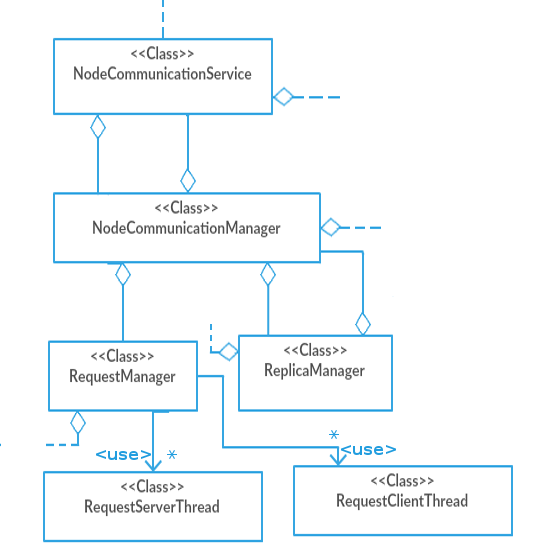
\includegraphics[scale=0.35]{core_communication_node}
\caption{Part of the UML class diagram, showing up relationships among classes in the core.communication.node subpackage}
\label{fig:class_diag_core.communication.node	}
\end{figure}

\paragraph{Message} A Message is the base interface for communications. Following the layout of the project, three further interfaces are defined, that inherits from Message: ClientMessage, NodeMessage and UpdateMessage, to deal respectively with client messages, node messages and database backup. 
\begin{itemize}
\item \textit{Message} Base interface: inplementing classes must provide methods to return the status (success, error, ...) and the type (put, get, ...) of the message.
\item \textit{ClientMessage} Interface that allows to retrieve the url inserted by the client.
\item \textit{GetMessage} Class that implements ClientMessage, it is used when GET requests are invoked by the client.
\item \textit{PutMessage} Class that implements ClientMessage, it is used when PUT requests are invoked by the client.
\item \textit{RemoveMessage} Class that implements ClientMessage, it is used when REMOVE requests are invoked by the client.
\item \textit{NodeMessage} Interface for the messages generated by the nodes from the client messages. Provides methods to retrieve the original url, the associated shortened url and the vector clock associated to those urls.
\item \textit{VersionedMessage} Class that implements the NodeMessage interface.
\item \textit{UpdateMessage} Interface used when portions of the database are sent to the backup node. Implementing classes must provide methods to put and get entries of the database in the message, check whether the UpdateMessage is full or empty, return the identifier of the sender node and tell whether this message is the first of a sequence of UpdateMessage. Indeed, the content of a backup is delivered by sending a sequence of UpdateMessages, and te first message may need some special treatment.
\item \textit{SizedBackupMessage} Class that implements the UpdateMessage interface. Its name means that it is involved in backup operations and that can carry only a limited amount of entries (indeed these messages have to be sent over UDP).
\end{itemize}

\subsubsection{The client module} 

\begin{figure}[t]
\centering
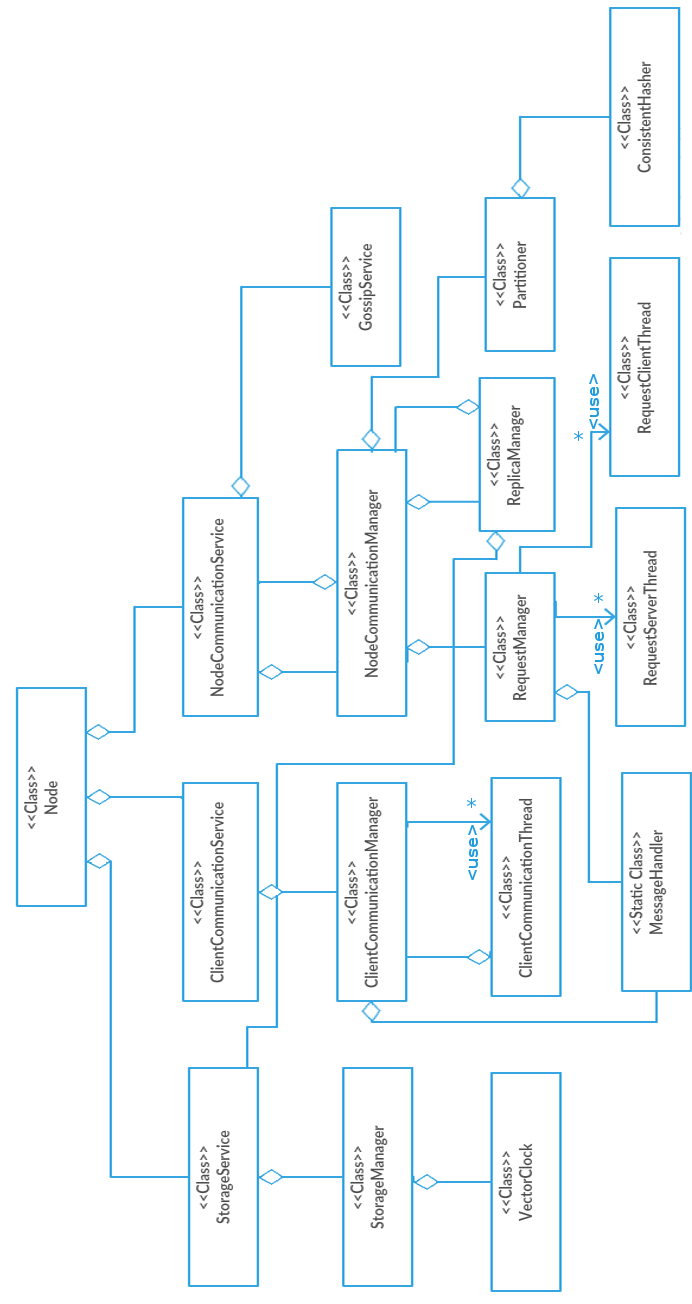
\includegraphics[scale=0.43]{core_diagram}
\caption{Uml Class Diagram of the core module. It is shown the internal composition of the node, which is the building block of the cluster. A node is made of a NodeCommunicationService, a ClientCommunicationService and a StorageService. In turn, these services rely on proper managers, who actually implement the functionalities of the services. Where omitted, cardinalities are 1.}
\label{fig:class_diag}
\end{figure}

\subsection{Use cases} 

\subsubsection{Management of a client request} 

\subsubsection{Replication of data} 

\section{Test}

\subsubsection{Correct behaviour of put, get, remove} 

\subsubsection{Self-healing } 
\todo[inline]{ (Primary failure) Show that in case of primary failure the system still works correctly, without needing any manual intervention}


\subsubsection{Conflict Resolution} 

\subsubsection{Load Balancing} 
\todo[inline]{Tweak the number of virtual nodes to show that more powerful machines can actually be assigned more items} 


\section{Future work} 
\begin{itemize}
\item Hash function for the url shortener. \todo[inline]{32 bit hash function allows too few urls; and in that case find another method to translate sequence of bytes into allowed charactes [A-Za-z0-9]}
\end{itemize}

\end{document}
